\chapter{Background and Fundamentals}
\label{chap:background}

\chapterquote{I have got my result, but I do not know yet how to get it. 
}{Carl Friedrich Gauss}
This chapter is devoted to introducing the  pre-requisite knowledge necessary to grapple with the material in subsequent sections. The subject matter of this dissertation lies at the intersection of several mathematical topics, ensuring that any treatment  of the material will give rise to notational challenges. Nevertheless, we have strived---courageously, in the author's unbiased opinion---to use standard notation wherever possible in the hopes that readers familiar with spectral graph theory may skip this background material without losing the plot. Omitted proofs  can be found  in  Appendix~\ref{sec:app_proofs_background}. 


\section{General Notation}
\label{sec:background_general}
We use the standard notation for sets of numbers: $\R$ (reals), $\N$ (naturals), $\Z$ (integers).  We use the subscript $\geq 0$ (resp., $>0$) to restrict a relevant set to its non-negative (resp., positive) elements ($\R_{\geq 0}$, for example). 
We will often introduce new notation or definitions by using the notation $\equiv$. The complement of a set $U$ (with respect to what will be clear from context) is denoted $U^c$. 
Given a set of scalars $K$, we let $K^{n\times m}$ denote the set of $n\times m$ matrices ($n$ rows and $m$ columns) with elements in $K$. Matrices will typically be denoted by uppercase letters in boldface, e.g., $\Q\in K^{n\times m}$. Matrices will also often be referred to as linear transformations and written, for example, as $\Q:K^m \to K^n$. 
We let $\Q(i,\cdot)$ (resp., $\Q(\cdot,i)$) denote the $i$-th row (resp., column) of the matrix $\Q$. 
For a set $U$, $K^U$ denotes the set of all functions from $U$ to $K$.  Elements of $K^U$ are also called vectors. For any $n\in\N$, set $[n]\equiv \{1,2,\dots,n\}$. As usual, we let $K^n=K^{[n]}$. Vectors will typically be denoted by lowercase boldcase letters. Lowercase  greek letters will often be used for scalars. It will often  be intuitively useful to identity vectors with their endpoints, rather than the traditional ``arrow'' originating from the origin. When this is the case, we will often use the word point instead of vector. We emphasize that they are formally the same object. 

For $n\in \N$, let $\zero_n\in\R^n$ and $\one_n\in\R^n$ be the vectors of all zeroes and all ones. Let $\I_n$ and $\J_n$  refer to the $n\times n$ identity matrix and all-ones matrix respectively (so $\J_n=\one_n\one_n^\tp)$. When the dimension $n$ is understood from context, will typically omit it as a subscript. We use $\chi(E)$ or $\chi_E$ as the indicator of an event $E$, i.e., $\chi(E)=1$ if $E$ occurs, and 0 otherwise. For example, $\chi(i\in U)=1$ if $i\in U$, and 0 if $i\in U^c$.  Similarly, for $U\subset K$,  $\bchi_U\in\R^K$ is the indicator vector of the set $U$, so $\bchi_U(i)=\chi(i\in U)$. 
By $\diag(x_1,x_2,\dots,x_n)$ we mean the $n\times n$ matrix $\Q$ entries $\Q(i,i)=x_i$ and $\Q(i,j)=0$ for $i\neq j$. Given vectors $\v_1,\dots,\v_n$, we will often denote by $(\v_1,\dots,\v_n)$ the matrix whose $i$-th column is $\v_i$. The $i$-th coordinate of a vector $\x$ will be denoted either by $\x(i)$ or simply $x(i)$. We trust this will not be overly confusing.  For $1\leq p<\infty$, the \emph{$p$-norm} of $\x\in \R^d$ is 
$\norm{\x}_p = \bigg(\sum_{i=1}^d x_i^p\bigg)^{1/p}$,
while the \emph{0-norm} of $\x$ is the number of non-zero entries of $\x$, and is denoted by $\norm{\x}_0$.  Given a vector or matrix, we use the superscript $t$ to denote it's transpose, i.e.,, given $\Q$, $\Q^t$ is defined as $\Q^t(i,j) = \Q(j,i)$. The standard inner product on $\R^d$ is denoted as $\la\cdot,\cdot\ra$, that is, $\la \x,\y\ra = \sum_i x(i)y(i)$. Elementary properties of the inner product will often be used without justification, such as its bilinearity: $\la \x,\alpha\y_1+\y_2\ra  = \la \x,\alpha\y_1\ra + \la \x,\y_2\ra$ for $\alpha\in\R$.  We will sometimes use the notation $\perp$ to mean ``orthogonal to'', so $\x\perp\y$ iff $\la\x,\y\ra=0$. We will often use the shorthand ``iff'' to mean ``if and only if''. We use $\delta_{ij}$ to denote the Kronecker delta function, i.e., $\delta_{ij} = 1$ if $i=j$ and 0 otherwise. We may sometimes include a comma and write $\delta_{i,j}$. 

A set $\X\subset\R^m$ is \emph{convex} if for all $\x,\y\in\X$ and $\lambda\in(0,1)$, $\lambda\x + (1-\lambda)\y\in \X$. 
The \emph{convex hull} of a finite set of points $X=\{\x_1,\dots,\x_k\}\subset \R^n$ is 
\begin{equation}
\label{eq:conv(X)}
\conv(\X) \equiv \bigg\{\sum_\ell \alpha_i\x_i: \sum_\ell \alpha_i = 1, \;\alpha_i\geq 0\bigg\},
\end{equation}
or equivalently, the smallest convex set containing $X$~\cite{grunbaum1967convex}. We will often denote the \emph{squared distance matrix of $\X$} by $\D(\X)\in\R^{|\X|\times |\X|}$,  whose entries are given by $\D(\x,\y) = \norm{\x-\y}_2^2$.  


\section{Linear Algebra}
\label{sec:background_linear} 
We assume familiarity with the basic linear algebraic notions---determinants, dimension, span, etc. We use the standard notation for these---$\det$, $\dim$, $\spn$, etc. All relevant background material can be found in a standard reference, e.g. \cite{axler1997linear}. 
We begin by stating a well-known but substantial result first proved by Cauchy (see \cite{hawkins1975cauchy} for the relevant history), which initiated the systematic study of the spectrum of matrices and which underpins the results in this dissertation. 

\begin{theorem}[Spectral Theorem for real matrices]
	\label{thm:spectral_theorem}
	Every real, symmetric $n\times n$ matrix has a set of $n$ orthogonal eigenvectors and real eigenvalues.  
\end{theorem}

Next we state a result which will underpin our construction of the ``dual simplex'' in Section \ref{sec:background_dual_simplex}. 

\begin{lemma}
\label{lem:bi-orthogonal_bases}
Let $\v_1,\dots,\v_k$ be a set of linearly independent vectors in $\R^n$. There exists a set of vectors, $\u_1,\dots,\u_k$ such that $\la \v_i,\u_j\ra = \delta_{ij}$ for all $i,j\in[k]$. The collections $\{\v_i\}$ and $\{\u_i\}$ are called \emph{biorthogonal} or \emph{dual bases}.  
\end{lemma}

Given the set $\{\v_i\}$ of linearly independent vectors, the complementary set $\{\u_i\}$ given by Lemma \ref{lem:bi-orthogonal_bases} is called the \emph{sister} or \emph{dual set to $\{\v_i\}$}. If $\{\v_i\}$ constitutes a basis of the underlying space, then we might call $\{\u_i\}$ the \emph{sister} or \emph{dual basis}.  We present a simple observation which will be useful in later sections. 

\begin{observation}
\label{obs:bi-orthogonal_unique}
Let $\{\v_1,\dots,\v_n\}\subset\R^n$ be a set of linearly independent vectors. The sister basis given by Lemma \ref{lem:bi-orthogonal_bases} is unique. 
\end{observation}

Let $\M\in\R^{n\times n}$. We recall that a vector $\eig$ satisfying $\M\eig=\lambda\eig$ is an \emph{eigenvector} of $\M$, and call $\lambda$ the associated \emph{eigenvalue}. It's clear that if $\eig$ is an eigenvector then so it $c\eig$ for any constant $c\in \R$. If $\M$ is real and symmetric, then the Spectral theorem dictates that there exists an orthonormal basis consisting of eigenvectors $\{\eig_1,\eig_2,\dots,\eig_n\}$ of $\M$ whose corresponding eigenvalues $\{\lambda_1,\dots,\lambda_n\}$ are all real. Let $\Eig=(\eig_1,\eig_2,\dots,\eig_n)$ be the matrix whose $i$-th column is the $i$-th eigenvector of $\M$, and set $\Eval=\diag(\lambda_1,\dots,\lambda_n)$. Observe that 
\begin{equation}
\label{eq:eig_decomp}
\M\Eig=\M(\eig_1,\dots,\eig_n)=(\M\eig_1,\dots,\M\eig_n)=(\lambda_1\eig_1,\dots,\lambda_n\eig_n)=\Eig\Eval.
\end{equation}
Moreover, if $\{\eig_i\}_i$ are assumed to be orthonormal then $\Eval\Eval^\intercal=\I$ from which it follows from $\eqref{eq:eig_decomp}$ that \begin{equation}
    \label{eq:eig_decomp2}
    \M=\Eig\Eval\Eig^\tp = \sum_{i\in[n]}\lambda_i\eig_i\eig_i^\tp,
\end{equation}
which is called the \emph{eigendecomposition} of $\M$. 
If $\M$ obeys  $\x^\tp\M\x\geq 0$ for all  $\x\in\R^n$, then we  call $\M$ \emph{positive semidefinite (PSD)}. Importantly, if $\M$ is PSD, then its eigenvalues are non-negative. Indeed, with the  eigendecomposition of $\M$ as  above,  
\[0\leq \vp_k^\tp \M\vp_k =\sum_{i\in[n]}\lambda_i \vp_k^\tp\vp_i\vp_i^\tp\vp_k = \lambda_k\vp_k^\tp\vp_k\vp_k^\tp\vp_k=\lambda_k,\]
for any $k$ since $\{\vp_i\}$ are orthonormal. Thus,  if  $\M$ is PSD we define 
\begin{equation*}
    \M^{1/2} \equiv \Eig\Eval^{1/2}\Eig^\tp = \sum_{i\in[n]}\sqrt{\lambda_i}\vp_i\vp_i^\tp.
\end{equation*}
It's easily verified that $(\M^{1/2})^2 = \M$. The following basic  result will be useful; the proof can  be found in the appendix. 

\begin{lemma}
	\label{lem:rank(QtQ)}
	For any $\M:\R^n\to\R^m$, $\rank(\M) = \rank(\M^\tp\M)$. 
\end{lemma}

We conclude with a formula for  the determinant of the minor of an invertible matrix.  It is often referred to as (a special  case of) \emph{Sylvester's identity}~\cite{sylvester1851xxxvii}. We state the version described by Viktor Prasolov~\cite{prasolov1994problems}. 

\begin{lemma}
	\label{lem:sylvester}
	Let $\Q\in\R^{n\times n}$ have a non-zero determinant, and let $\emptyset\neq U\subsetneq[n]$. Then 
	\begin{equation}
	\label{eq:sylvester}
	\det(\Q^{-1}[U,U]) \det(\Q) = \pm \det(\Q[U^c,U^c]). 
	\end{equation}
\end{lemma}



\subsection{Pseudoinverse}
\label{sec:background_pseudoinverse}

If $\M$ is a singular matrix, a natural question to ask is whether there exists a matrix whose relationship to $\M$ ``approximates'', in some relevant sense, the relationship between a matrix and its inverse. This question  was asked and answered, on separate occasions, by both Elikam Moore and Sir Roger Penrose. Both discovered---originally Moore in 1921 and later Penrose in the 1950's---what is now known as the \emph{Moore-Penrose pseudoinverse} of a matrix~\cite{moore1920reciprocal, penrose1955generalized,penrose1956best}. It is defined as follows. 

\begin{definition}[Moore-Penrose pseudoinverse~\cite{barata2012moore}]
\label{def:pseudoinverse}
Let $\M\in\C^{n\times m}$ for some $n,m\in\N$. We call a matrix $\M^+\in\C^{m\times n}$ satisfying both
\begin{enumerate}
    \item[(i).] $\M\M^+\M=\M$ and $\M^+\M\M^+=\M^+$;
    \item[(ii).] $\M\M^+$ and $\M^+\M$ are hermitian, i.e., $\M\M^+=(\M\M^+)^\tp $, $\M^+\M=(\M^+\M)^\tp$; 
\end{enumerate}
the \emph{Moore-Penrose Pseudoinverse} of $\M$. 
\end{definition}

We will often drop the identifier ``Moore-Penrose'' and simply write that $\M^+$ is the pseudoinverse of $\M$. It's not immediate from  the definition, but the pseudoinverse of $\M$ has several desirable properties: When $\M$ is real, so is $\M^+$; $(\M^+)^+=\M$; $(\M^+\M)^\tp = \M^+\M$. Importantly, when $\M$ is invertible, then $\M^+=\M^{-1}$. Moreover, the pseudoinverse always exists: 

\begin{lemma}[\cite{barata2012moore}]
	\label{lem:pseudoinverse_properties}
Let $\M\in \C^{n\times m}$. The pseudoinverse  $\M^+$ of $\M$ exists and is unique. Moreover, the following properties hold: 
\begin{enumerate}
    \item[(i).] $\M\M^+$ is an orthogonal projector obeying $\range(\M\M^+)=\range(\M)$; and 
    \item[(ii).] $\M^+\M$ is an orthogonal projector obeying $\range(\M^+\M)=\range(\M^+)$. 
\end{enumerate}
\end{lemma}

Together, Definition \ref{def:pseudoinverse} and Lemma \ref{lem:pseudoinverse_properties} do not necessarily yield a way to obtain the pseudoinverse of a matrix $\M$. We  next demonstrate that when the eigendecomposition is known, we  can give a precise expression for the pseudoinverse. 

\begin{lemma}
\label{lem:pseudoinverse_eigendecomposition}
Suppose $\M\in\C^{m\times m}$ admits the eigendecomposition 
$\M=\sum_{i=1}^k \lambda_i \vp_i\vp_i^\tp$, 
where $\lambda_i$, $1\leq i\leq k$ are the non-zero eigenvalues of $\M$ with corresponding orthornomal eigenvectors $\vp_1,\dots,\vp_k$. Then the pseudoinverse of $\M$ is 
\begin{equation}
    \label{eq:pseudoinverse}
    \M^+=\sum_{i=1}^k \frac{1}{\lambda_i}\vp_i\vp_i^\tp.
\end{equation}
\end{lemma}


\section{Spectral Graph Theory}
\label{sec:background_spectral}

Similarly to  Section \ref{sec:background_linear}, the results in this section can be found in any self-contained reference on (spectral) graph theory (see e.g., \cite{spielman2009spectral,chung1997spectral}).

We begin with basic graph theory. 
We denote a \emph{graph} by a triple $G=(V,E,w)$ where $V$ is the \emph{vertex set}, $E\subset V\times V$ is the \emph{edge set} and $w:V\times V\to\R_{\geq0}$ (the non-negative reals) a \emph{weight function}. We let the domain of $w$ be $V\times V$ for convenience; for $(i,j)\notin E$ we have $w((i,j))=0$. We call $G$ \emph{unweighted} if $w((i,j))=\chi_{(i,j)\in E}$ for all $i,j$. In this case, we may omit the weight function and simply write $G=(V,E)$. 
Unless otherwise stated, $G$ will be undirected (edges do not have  directions) and connected (each vertex is reachable from every other vertex). 
We will typically take $V=[n]$ for simplicity. For a  vertex $i\in V$, we denote the set of its neighbours by 
\begin{equation}
\label{eq:delta(i)}
\partial_G(i) \equiv  \{j\in V:w(i,j)>0\},
\end{equation}
a set we call that \emph{neighbourhood} of $i$. The \emph{degree of $i$} if $\deg(i)\equiv |\partial(i)|$. The \emph{weight of $i$} if $w(i)\equiv \sum_{j\in \partial(i)}w(i,j)$. Note that if $G$ is unweighted, then $w(i)=\deg(i)$. If the degree of each vertex in $G$ is equal to $k$, we call $G$ a \emph{$k$-regular graph}. We call $G$ \emph{regular} if it is $k$-regular for some $k$. If $U\subset V$ contains only vertices with the same degree (resp., weight), we call it \emph{degree (resp., weight) homogeneous}. 
For a set of subset of vertices $U$, the \emph{volume of $U$} is 
\begin{equation}
\label{eq:volU}
\vol_G(U) \equiv \sum_{i\in U}w(i),
\end{equation}
and the volume of $G$ is $\vol(G) \equiv \vol_G(V(G))$. As usual, we will drop the subscript if the graph is clear from context. 
Owing to possible mental lapses and above average caffeine intake, we may sometimes abuse notation and extend the weight function $w$ to sets of edges or vertices by setting $w(A)=\sum_{a\in A}w(a)$. Thus, for instance, $w(U) = \vol(U)$, for $U\subset V$. (The more notation the better, right?) 

Given a subset $U\subset  V$, we write $G[U]$ to be the graph induced by $U$, i.e., $V(G[U])  = V\cap U$ and  $E(G[U]) = E \cap U \times U$. If a graph is connected  and acyclic (i.e., there is a unique path between each pair of vertices) we call it a \emph{tree}. It's well known that a tree on $n$ nodes has $n-1$ edges.  

As mentioned above, we will typically  work  with undirected graphs. In this case, we identify each tuple $(i,j)$ with its sister pair $(j,i)$. This implies, for example, that when summing over all edges $(i,j)\in E$ we are \emph{not} summing over all vertices and their neighbours. Indeed, this latter summation double counts the edges: $\sum_{(i,j)\in E}=\frac{1}{2}\sum_{i}\sum_{j\in\partial(i)}$. We will often write $i\sim j$ to denote an edge $(i,j)$; so, for example, $\sum_{i\sim j}=\sum_{(i,j)\in E}$. 

We will also appeal to the so-called ``handshaking lemma'' for unweighted graphs, which states that $\sum_i \deg_G(i) = 2|E(G)|$; easily verified with a counting argument. 


\subsection{Laplacian Matrices}
\label{sec:background_laplacian}
Here we introduce various matrices of graphs, including the Laplacian. See  the survey by Merris~\cite{merris1994laplacian} for an excellent overview of the Laplacian, and that by Mohar~\cite{mohar1991laplacian} for an overview of its spectrum. 


Let $G=(V,E,w)$ be a graph, with $V=[n]$ and $|E|=m$. 
Let $\W$ be the \emph{weight matrix} of $G$, i.e., $\W=\diag(w(1),w(2),\dots,w(n))$. 
The \emph{degree matrix} of $G$ is \[\diag(\deg(1),\deg(2),\dots,\deg(n)).\] The \emph{adjacency matrix} of $G$ encodes the edge relations, namely, $\A_G(i,j)=w((i,j))$ for all $i\neq j$, and $\A_G(i,i)=0$ for all $i$. Notice that (for undirected graphs) $\A_G$ is symmetric.  Note that if $G$ is unweighted, then $\W_G$ and the degree matrix are equivalent. 
The \emph{combinatorial Laplacian} of $G$ is the matrix 
\begin{equation}
\label{eq:L_G}
\L_G\equiv \W_G-\A_G.
\end{equation}
There are several useful representations of the Laplacian. Let $\L_{i,j}=w(i,j)(\chi_i-\chi_j) (\chi_i-\chi_j)^\tp\in \R^{V\times V}$, i.e., 
\[\L_{i,j}(a,b)=\begin{cases}
w(i,j)&a=b\in\{i,j\},\\
-w(i,j),&(a,b)=(i,j),\\
0,&\text{otherwise}.
\end{cases}\]
Then 
\begin{equation}
\label{eq:Lsum}
    \L_G=\sum_{i\sim j}\L_{i,j}.
\end{equation}
Another representation comes via the \emph{incidence matrix} of $G$, $\B_G\in \R^{E\times V}$, defined as follows. Place an arbitrary orientation on the edges of $G$ (say, for example, $(i,j)$ is directed from $i$ to $j$ iff $i<j$), and for an edge $e$, let $e^-\in V$ denote the vertex at which $e$ begins, and $e^+$ the vertex at which it ends. Set 
\begin{equation}
\label{eq:B_G}
\B_G(e,i)=\begin{cases}
1&\text{if }i=e^-,\\
-1&\text{if }i=e^+,\\
0&\text{otherwise},
\end{cases}
\end{equation}
or, equivalently, $\B_G(e,i) = (\chi_{(i=e^-)}-\chi_{(i=e^+)})$. Then,
\begin{equation*}
   ( \B_G^\tp\W_G\B_G)(i,j)=\sum_{e\in E} \B_G^\tp(i,e)\B_G(e,j)=\sum_{e\in E}w(e)(\chi_{i=e^-}-\chi_{i=e^+})(\chi_{j=e^-}-\chi_{j=e^+}).
\end{equation*}
Let $\alpha(e)=(\chi_{i=e^-}-\chi_{i=e^+})(\chi_{j=e^-}-\chi_{j=e^+})$. If $i=j$, then $\alpha(e)=1$ iff $e$ is incident to $i$, and 0 otherwise. If $i\neq j$, then $\alpha(e)=1$ for $e=(i,j)$ and 0 otherwise, regardless of whether $i=e^-$ and $j=e^+$ or vice versa (this is what ensures that the orientation we chose for the edges is inconsequential). Consequently, 
\begin{align*}
(\B_G^\tp\W_G\B_G)(i,j) = 
\begin{cases}
\sum_{e\ni i} w(e),&\text{if } i=j,\\
-w((i,j)),&\text{otherwise}, 
\end{cases}
\end{align*}
which is precisely $\L_G(i,j)$. That is, we have 
 \begin{equation}
 \label{eq:L=BTB}
 \L_G=(\W_G^{1/2}\B_G)^\tp(\W_G^{1/2}\B_G).
 \end{equation}
 We associate with $\L_G$ the quadratic form $\Lop_G:\R^V\to \R$ which acts on functions $\f:V\to \R$ as $f\xmapsto{\Lop_G} \f^\tp \L_G \f$.
The Laplacian quadratic form will be crucial in our study of the geometry of graphs. Luckily for us then, its action on a vector is captured by an elegant closed-form formula. 
Computing 
$\L_{i,j}\f = w(i,j)(\bchi_i -\bchi_j)(\bchi_i-\bchi_j)^\tp \f = w(i,j)(\f(i)-\f(j))(\bchi_i-\bchi_j)$,
we find that 
$\f^\tp \L_{i,j} \f = w(i,j)(\f(i)-\f(j))^2$.
Therefore, applying Equation \ref{eq:Lsum} yields 
\begin{equation}
\label{eq:Lf}
    \Lop_G(\f) = \f^\tp \bigg(\sum_{i\sim j} \L_{i,j}\bigg) \f = \sum_{i\sim j}\f^\tp \L_{i,j} \f= \sum_{i\sim j} w(i,j)(\f(i)-\f(j))^2.
\end{equation}

Another Laplacian matrix associated with $G$ is the \emph{normalized Laplacian}, given by 
\begin{equation}
\label{eq:Ln_G}
    \Ln_G = \W_G^{-1/2} \L_G\W_G^{-1/2} = \I - \W_G^{-1/2} \A_G\W_{G}^{-1/2}.
\end{equation} 
The normalized Laplacian is intimately related to various  phenomena, most notable random walks on the graph~\cite{chen2007resistance,chung1997spectral}. To investigate $\Ln_G$ we may carry out a similar procedure to above. In particular, if we define $\Ln_{i,j}=\W_G^{-1/2} \L_{i,j}\W_G^{-1/2}$ then we obtain the equivalent of Equation~\eqref{eq:Lsum} for the normalized Laplacian:
\begin{equation}
\label{eq:Lnsum}
    \Ln_G = \sum_{i\sim j}\Ln_{i,j}.
\end{equation}
Likewise, 
\begin{equation*}
   \W_G^{-1/2}\Bn_G^\tp \W_G\Bn_G\W_G^{-1/2} =  \W_G^{-1/2}\L_G\W_G^{-1/2}=\Ln_G
\end{equation*}
As we've done here, we will typically emphasize the associate of elements associated to the normalized Laplacian with a hat.
Using Equation~\eqref{eq:Lnsum}, we see that 
the quadratic form $\Lnf_G$ associated with $\Ln_G$ acts as 
\begin{equation}
\label{eq:Lnf}
    \Lnf_G(\f) = \sum_{i\sim j} w(i,j)\bigg(\frac{\f(i)}{\sqrt{w(i)}}-\frac{\f(j)}{\sqrt{w(j)}}\bigg)^2.
\end{equation}

We now discuss  the spectrum of $\L_G$ and $\Ln_G$. Both the combinatorial and normalized Laplacian of an undirected graph $G$ are real, symmetric matrices. By the spectral theorem therefore, they both admit a basis of orthonormal eigenfunctions corresponding to real eigenvalues. 

\begin{lemma}
	\label{lem:laplacian_props}
	Let $G=([n],E)$ be a connected graph. Then  $\ker\L_G=\spn(\one)$ and $\ker\Ln_G=\spn(\sqrt{\w})$. Moreover, both  $\L_G$ and $\Ln_G$ have a single zero eigenvalue (with corresponding eigenvector $\one$ and $\sqrt{\w}$, respectively); all other eigenvalues are strictly positive. 
\end{lemma}


We  end this section by discussing two properties of graph Laplacians. The first is  their pseudoinverse relationships, and the second is the remarkable link between the eigenvalues of the combinatorial  Laplacian and spanning trees of the graph. 

\paragraph{Pseudoinverse of \texorpdfstring{$\L_G$}{the combinatorial} and \texorpdfstring{$\Ln_G$}{normalized Laplacian}.}
Since $\L_G$ and $\Ln_G$ are both symmetric, $\range(\L^\tp)=\range(\L)=\R^n \setminus \ker(\L)=\R^n \setminus \spn(\{\one\})$, and $\range(\Ln^\tp)=\range(\Ln)=\R^n \setminus \ker(\Ln)=\R^n \setminus \spn(\{\W^{1/2}\one\})$. It follows by Lemma \ref{lem:pseudoinverse_properties} that the pseudoinverses of these two Laplacians satisfy
\begin{equation}
\label{eq:LL^+}
\L_G\L_G^+ = \L_G^+\L_G = \I - \frac{1}{n}\one\one^\tp,,
\end{equation}
i.e., the projection onto $\spn(\one)^\perp$, and 
\begin{equation}
\label{eq:LnLn^+}
\Ln_G\Ln_G^+ = \Ln_G^+\Ln_G = \I - \frac{1}{\vol(G)}\W_G^{1/2}\one(\W_G^{1/2}\one)^\tp = \I-\frac{1}{\vol(G)}\sqrt{\w}\sqrt{\w}^\tp,
\end{equation}
the projection onto $\spn(\w)^\perp$, where $\sqrt{\w}=(\sqrt{w(1)},\dots,\sqrt{w(n)})$. Note that the denominator in \eqref{eq:LnLn^+} is $\vol(G)$ instead of $n$ to ensure the result is a projection matrix. Put $\vb{P} = \I-\frac{1}{\vol(G)}\sqrt{\w}\sqrt{\w}^\tp$. Then 
\begin{align*}
\vb{P}^2 = \I - \frac{2}{\vol(G)}\sqrt{\w}\sqrt{\w}^\tp + \frac{1}{\vol(G)^2}\sqrt{\w}\sqrt{\w}^\tp\sqrt{\w}\sqrt{\w}^\tp = \vb{P},
\end{align*}
since $\sqrt{\w}^\tp\sqrt{\w}= \vol(G)$. 



\paragraph{Kirchoff's  Theorem. }
A  \emph{spanning tree} of a graph $G$ is a connected subgraph $T$ of $G$ with $V(T)=V(G)$ and $|E(T)| = |V(T)|-1$. That  is, $T$ contains the minimum number of edges possible to connect all vertices of $G$.   
We will make use  of the following Theorem, often  called the \emph{Kirchhoff Tree Theorem}, named after Gustav Kirchhoff for the work done in \cite{Kirchhoff1847}. It was first stated in its most familiar form by Maxwell~\cite{maxwell1873treatise}. We use the formulation found in~\cite{chaiken1978matrix}. 

\begin{theorem}
	\label{thm:matrix_tree_theorem}
	Let $G=(V,E,w)$ be a connected, undirected graph. Let $\L$ be $G$'s combinatorial Laplacian matrix. Then for all $i,j\in[n]$, 
	\[\Gamma_G = (-1)^i(-1)^j \det(\L_{-i,-j}) = \frac{1}{n}\prod_{i=1}^{n-1} \lambda_i,\]
	where $\lambda_1,\dots,\lambda_{n-1}$ are the non-zero eigenvalues of $G$, $\L_{-i,-j}$ is the matrix obtained by removing the $i$-th row and $j$-th column of $\L_G$, and $\Gamma_G$ is the weight of all spanning trees of $G$.  
\end{theorem}

\begin{remark}
	The  $\mathfrak{T}$ be the set of all spanning trees of a graph $G$. By the ``weight of all spanning trees'', we mean that
	\begin{equation}
	\label{eq:Gamma_G}
	\Gamma_G = \sum_{T\in \mathfrak{T}} \prod_{i\in  V(T)} w_G(i).
	\end{equation}
	Thus, for $G$ unweighted, $\prod_{i\in V(T)}w_G(i)=1$ so $\Gamma_G$ simply counts the number of spanning trees. 
\end{remark}




\section{Electrical Flows}
\label{sec:background_er}

One of  the most successful physical interpretations of a graph arises from considering it as an electrical network~\cite{ellens2011effective,tetali1991random}. 
We imagine placing a resistor of resistance $1/w(i,j)$ on each edge $(i,j)\in E(G)$. Injecting current at one or more of the vertices results in an \emph{electrical flow} in the graph. While this physical interpretation  is intuitively useful, it is  not necessary for understanding  the notions of electrical flows. Consequently, we move a more involved discussion on electrical flows to Appendix~\ref{sec:app_er} and present only the required definitions  and results here. The key concept is that of the ``effective resistance'' between  two vertices:  


\begin{definition}
	\label{def:effective_resistance}
	The \emph{effective resistance} between nodes $i$ and $j$ is $\effr(i,j) \equiv \Lf_G^+(\bchi_i-\bchi_j)$, and the \emph{effective resistance matrix of $G$} is the matrix $\Reff_G$ with entries $\Reff_G(i,j)=\effr(i,j)$. The \emph{total effective resistance in the graph } is the quantity $\Rtot_G\equiv \frac{1}{2}\one^\tp\Reff_G\one$. 
\end{definition}

We can relate the entries of the pseudoinverse Laplacian with the effective resistance as follows.
\begin{lemma}
	\label{lem:er_props}
	For any graph $G$, $\Reff_G = \one \u ^\tp + \u\one^\tp - 2\L_G^+$ where $\u=\diag(\L_G^+(i,i))$. Moreover, for all $i,j$ (including $i=j$), 
	\begin{equation}
	\label{eq:L^+(i,j)}
	\L_G^+(i,j) = \frac{1}{2n}\bigg(\sum_{k\in[n]}\effr(i,k)+\effr(j,k)\bigg) - \frac{1}{2}\effr(i,j) -\frac{\Rtot_G}{n^2}.
	\end{equation}
\end{lemma}




\section{Simplices}
\label{sec:background_simplices}

Finally we reach what is our main object of study. We begin by describing a  relationship  among a set  of vertices which,  roughly speaking,  generalizes the notion of ``non-collinearity'' to  higher dimensions. We are then able to properly define a simplex and its dual. We end the section by briefly discussing several  of the angles in a simplex. 

\paragraph{Affine Independence.}
In order to properly define simplices, we need to define the  notion of ``affine independence'' between  points.  In $\R^2$, for example, such a relationship characterizes the sets of three points which describe a triangle. See Figure~\ref{fig:affine_independence} for an  illustration of affine dependence and independence.  


\begin{definition}
	\label{def:affine_independence}
A set of points $\x_1,\dots,\x_k$ are said to be \emph{affinely independent} if the only solution to $\sum_{i\in[n]}\alpha_i\x_i=\zero$ with $\sum_{i\in [n]}\alpha_i=0$ is $\alpha_1=\dots=\alpha_n=0$. 
\end{definition}

Perhaps a more useful characterization of affine independence is the following. 

\begin{lemma}
	\label{lem:affine-linearly-independent}
	The set $\{\x_1,\dots,\x_k\}$ is affinely independent iff for each $j$, $\{\x_j-\x_i\}_{i\neq j}$ is linearly independent. 
\end{lemma}

The following lemma demonstrates that if we form a matrix of size $n-1\times n$ from the column vectors of $n$  affine independent vectors, then this matrix has full rank. Moreover, we may assume that the linear combination of the vectors is in fact an \emph{affine combination}, in the  following sense. 

\begin{lemma}
	\label{lem:barycentric_coeffs}
	Let $\{\x_1,\dots,\x_n\}\subset\R^{n-1}$ be affinely independent, and let  $\y\in\R^{n-1}$ be arbitrary. Then there exists coefficients $\{\alpha_i\}\subset\R$ obeying $\sum_{i\in[n]}\alpha_i=1$ such that $\y=\sum_{i\in[n]}\alpha_i\x_i$. 
\end{lemma}

\paragraph{The simplex.} 
We jump straight into the definition; see Figure~\ref{fig:simplices} for several examples. 
\begin{figure}
	\centering
	\begin{minipage}{0.45\textwidth}
		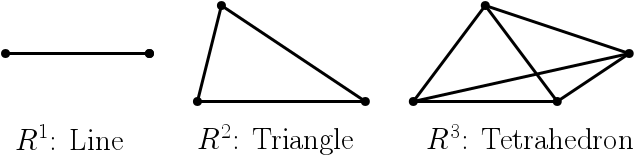
\includegraphics[scale=0.6]{simplices}
		\subcaption{}
		\label{fig:simplices}
	\end{minipage}
	\hspace{0.08\textwidth}
	\begin{minipage}{0.45\textwidth}
		\flushright
		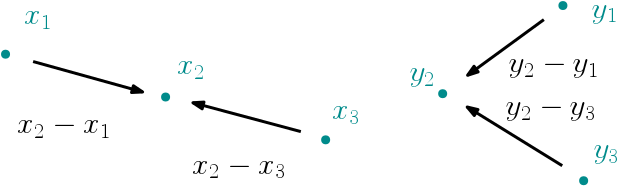
\includegraphics[scale=0.6]{affine_independence}
		\subcaption{}
		\label{fig:affine_independence}
	\end{minipage}
	\caption{(a) Simplices in dimensions one, two, and three. We wish the reader luck in visualizing a simplex (or anything really) in more than three dimensions. (b) Example of affine dependence and independence.  Here $x_1,x_2,x_3$ are not affinely independent, as evidenced by the fact that $x_2-x_1$ and $x_2-x_3$ are parallel. $y_1,y_2,y_3$ on the other hand, are affinely independent; one can easily visualize the triangle formed by their convex hull. We emphasize that the arrows representing the difference between two vectors, e.g., $x_2-x_1$, represent their \emph{direction only} and  not their absolute position.} 
	\label{fig:simplex+independence}
\end{figure}


\begin{definition}
\label{def:simplex}
A \emph{simplex} $\ssplx$ in $\R^{n-1}$ is the convex hull of $n$ affinely independent vectors $\sv_1,\dots,\sv_n$. That is, $\splx=\conv(\bgamma_1,\dots,\bgamma_n)$.  
\end{definition}

If we gather the vertices of the simplex $\ssplx$ into the \emph{vertex matrix} $\Sv=(\sv_1,\dots,\sv_n)$ whose columns are the vertex vectors of $\ssplx$, then we can write the simplex as 
\begin{equation*}
    \ssplx = \{\Sv \x:\x\geq \zero, \; \norm{\x}_1=1\}.
\end{equation*}
Given a point $\p=\Sv\x\in\splx$, $\x$ is called the \emph{barycentric coordinate} of $\p$.  

As is illustrated in two and three dimensions by the triangle and the tetrahedron, the projection of the simplex onto spaces spanned by subsets of its vertices yields simplices of lower dimensions. Let $U\subset [n]$. The \emph{face of $\ssplx$ corresponding to $U$} is 
\begin{equation}
\label{eq:T_U}
    \ssplx\restriction_U \equiv \{\Sv\x: \x\geq 0,\;\norm{\x}_1=1,\;x(i)=0\text{ for all }i\in U^c\}.
\end{equation}
If $|U|=n-1$, we call $\ssplx_U$ a \emph{facet}. Figure~\ref{fig:faces} illustrates a two-dimensional   facet and one-dimensional  face of a simplex in $\R^3$. The following observation demonstrates that $\splx\restriction_U$ is a well-defined simplex. 
\begin{observation}
	\label{obs:subset_affinely_independent}
	Any subset of an affinely independent set of vectors is again affinely independent. 
\end{observation}

Trusting the reader's capacity for variation, depending on the situation we may adopt different notation for the faces of a simplex. Oftentimes the vertical restriction symbol will be dropped and we will write only $\splx_U$; other times we will write $\splx[U]$, especially when the space reserved a subscript is being used for other purposes. 

In  our study of simplices we will be mainly concerned with their relative properties (e.g., volume, angles, shape, etc.) as opposed to their absolute  positions in space. Thus, it will often  be convenient to identity simplices which share the same relative properties, but are simply rotated and /or translated versions of one  another. We will call  such simplices \emph{congruent},  or occasionally \emph{isomorphic}. 
Unfortunately for notational simplicity, it will be  required to  sometimes differentiate between simplices  which are congruent by translation only, and simplices which are congruent by translation \emph{and} rotation. Let us  call the former type of congruence \emph{translational congruence}. We will continue to  call the latter simply congruence. Thus, the set of translationally congruent simplices to a simplex $\ssplx$ is a subset of  those simplices which are congruent to $\ssplx$. 
We use the symbol $\cong$ to denote translational congruency between simplices; so $\ssplx_1\cong\ssplx_2$ iff $\Sv(\splx_1)=\Sv(\splx_2) + \balpha\one^\tp$ for some $\balpha\in\R^{n-1}$. We use $\cong^\rot$  to denote general   congruency; so  $\ssplx_1\cong^\rot\ssplx_2$ iff  $\Sv(\ssplx_1)=\Q\Sv(\ssplx_2) + \balpha\one^\tp$ for some rotation matrix $\Q$  and $\balpha\in\R^{n-1}$. 
We will  also define two congruence classes of simplices. Put
\begin{equation}
\label{eq:[ssplx]}
[\ssplx] \equiv \{\ssplx': \ssplx'\cong\ssplx\},\quad \text{and} \quad [\ssplx]^\rot\equiv \{\ssplx':\ssplx'\cong^\rot\ssplx\}.
\end{equation}.

A brief note now on nomenclature. We will typically  use the symbol $\ssplx$ to denote an arbitrary simplex. Later, we will use the symbol $\splx$  to denote  the simplex associated  to a  graph. In  this way we hope to provide a clear separation between those statements which hold for general simplices and those which hold for simplices of a graph. 


\paragraph{Centroids and altitudes.}
Two fundamental objects related to a simplex are its centroids and altitudes (Figure~\ref{fig:faces+altitudes}). The \emph{centroid} of a simplex is the point 
\begin{equation}
\label{eq:centroid}
\cent(\ssplx) \equiv \frac{1}{n}\Sv \one = \frac{1}{n}\sum_{i\in[n]}\bgamma_i.
\end{equation} 

The centroid of a simplex can be thought of as its centre of mass, assuming that weight is distributed evenly across its surface. 
We can also of course discuss  the  centroid of a face $\ssplx_U$, which is $\cent(\ssplx_U) = |U|^{-1}\Sv\bchi_U$. 
The \emph{altitude between faces $\ssplx_U$ and $\ssplx_{U^c}$} is a vector which lies in the orthogonal complement of both $\splx_U$ and $\splx_{U^c}$ and points from one face to the other. 
We denote the altitude pointing from $\splx_{U^c}$ to $\splx_{U}$ as $\alt_(\splx_U)$. We can write the altitude as $\alt_U=\p-\q$ for some $\p\in \splx_{U^c}$ and $\q\in\splx_{U}$, and thus as $\Sv(\x_{U^c}-\x_{U})$ where $\x_{U^c}$ and $\x_{U}$ are the barycentric coordinates of $\p$ and $\q$. 

\textbf{Nota Bene:} While  we conceptualize of the altitude $\alt(\ssplx_U)$ as pointing from $\ssplx_U$  to  $\ssplx_{U^c}$, we  remark that since we are working in  $\R^{n-1}$  as  a vector  space,  $\alt(\ssplx_U)$ still ``begins'' at  the origin. 

\begin{figure}
	\centering
	\begin{minipage}{0.45\textwidth}
	\centering
	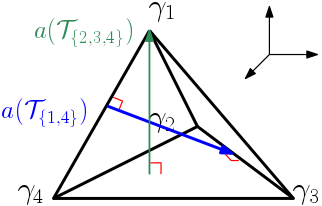
\includegraphics[scale=0.5]{altitudes}
	\subcaption{ }
	\label{fig:altitudes}
	\end{minipage}
\hspace{0.08\textwidth}
\begin{minipage}{0.45\textwidth}
	\centering
	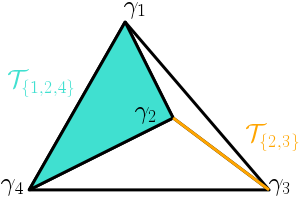
\includegraphics[scale=0.5]{faces}
	\subcaption{}
	\label{fig:faces}
\end{minipage}
\caption{(a) The \emph{directions} of altitudes in a simplex. We emphasize that the arrows do not represent the actual altitudes themselves, which  are  vectors and hence originate at the origin. (b) A one  ($\ssplx_{\{2,3\}}$) and two ($\splx_{\{1,2,4\}}$) dimensional face of a three dimensional simplex. }
\label{fig:faces+altitudes}
\end{figure}

\paragraph{Centred  simplex.}
In later sections it will be convenient to work with a translated copy of a given simplex which is centred at the origin. Accordingly, given any simplex $\ssplx$ with vertices $\{\sv_i\}$, we let $\ssplx_0$ denote the simplex with vertices $\{\sv_i - \cent(\ssplx)\}$. Note that $\ssplx_0\in[\ssplx]$. It's clear that the centroid of $\ssplx_0$ is the origin: 
\begin{align*}
\cent(\ssplx_0) 
&= \frac{1}{n}(\sv_1-\cent(\ssplx),\;\dots\;\sv_n-\cent(\ssplx))\one \\
&= \frac{1}{n}(\sv_1\;\dots\;\sv_n)\one - \frac{1}{n}(\cent(\ssplx)\;\dots\;\cent(\ssplx))\one = \cent(\ssplx) - \cent(\ssplx)=\zero.
\end{align*}

We solidify the concept with a definition. 

\begin{definition}
	\label{def:centred_simplex}
	Given a simplex $\ssplx$, the unique (up to rotation and translation) simplex with vertex matrix $\Sv(\ssplx) - (\cent(\ssplx)\;\dots\;\cent(\ssplx))$ centred at the origin is called the \emph{canonical (or centred) simplex corresponding to $\ssplx$} and is denoted $\ssplx_0$. 
\end{definition}

We may also refer to $\ssplx_0$ as the \emph{centred version of $\ssplx$} in order  spare  the author the agony induced by writing out the complete  sentence ``corresponding to the simplex $\ssplx$''. 

 

\subsection{Dual Simplex}
\label{sec:background_dual_simplex}

\begin{figure}
	\centering
	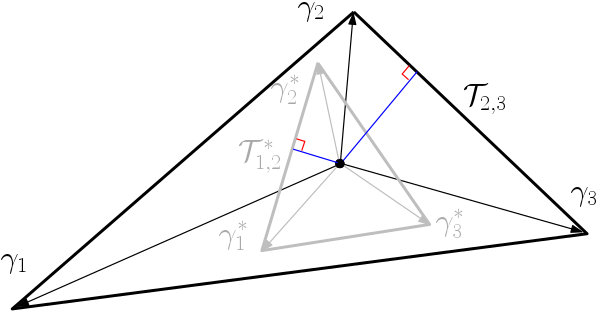
\includegraphics[scale=0.4]{dual_simplex}
	\caption{An example of a simplex $\ssplx\subset\R^2$ (in black) and its dual, $\ssplx^\du$  (in gray).  The blue lines serve to emphasize the  fact that the dual vertex $\bgamma_1^\du$ is orthogonal to the face $\ssplx_{2,3}$ just as $\bgamma_3$ is to $\ssplx^\du_{1,2}$. }
	\label{fig:dual_simplex}
\end{figure}
Here we introduce the notion of the dual simplex of a given simplex. Even  though we provide a novel treatment  of  the object, the proofs in this section   are  relatively elementary. As such, they have been moved to Appendix~\ref{sec:app_proofs_background}. 

Let $\Sv=(\bgamma_1,\dots,\bgamma_n)\in\R^{n-1\times n}$ be the vertex matrix of a simplex $\ssplx\subset\R^{n-1}$. For each $i\in[n-1]$, put $\v_i=\bgamma_n-\bgamma_i$. Then $\{\v_1,\dots,\v_{n-1}\}$ is a linearly independent set, and thus admits a sister basis $\{\bgamma^\du_1,\dots,\bgamma^\du_{n-1}\}$ which together form biorthogonal bases of $\R^{n-1}$ (Lemma \ref{lem:bi-orthogonal_bases}). Put $\bgamma^\du_n = -\sum_{i=1}^{n-1}\bgamma^\du_i$.  

\begin{claim}
	\label{claim:affine_independence}
The set 
$\{\bgamma^\du_1,\dots,\bgamma^\du_n\}$ is affinely independent. 
\end{claim}

Therefore, the set $\{\bgamma^\du_1,\dots,\bgamma^\du_n\}$ determines a simplex, which we call the \emph{dual simplex} of $\ssplx$. Of course, it would highly suboptimal if the notion of a dual simplex depended on the labelling of the vertices of $\ssplx$. More specifically, we defined the vertices of the dual simplex $\bgamma^\du_i$ with respect to the vectors $\{\bgamma_i-\bgamma_n\}$. It is not clear a priori whether the vertices of the dual simplex would change were we to relabel the indices of $\{\bgamma_i\}$. In fact, they do not---the demonstration of which is the purpose of the following lemma. 

\begin{lemma}
	\label{lem:dual_vertices_well-defined}
	Let $\{\bgamma_1,\dots,\bgamma_n\}$ be a set of affinely independent vectors. Fix $k\in [n-1]$ and define $\v_i=\bgamma_i-\bgamma_n$ for $i\in[n-1]$ and $\u_i=\bgamma_i-\bgamma_k$ for $i\in[n]\setminus\{k\}$. If $\{\bgamma^\du_1,\dots,\bgamma^\du_{n-1}\}$ is the sister basis to $\{\v_1,\dots,\v_{n-1}\}$ and $\bgamma^\du_n = -\sum_{i=1}^{n-1}\bgamma_i$, then $\{\bgamma^\du_1,\dots,\bgamma^\du_{k-1},\bgamma^\du_{k+1},\dots,\bgamma^\du_{n}\}$ is the sister basis to $\{\u_1,\dots,\u_{k-1},\u_{k+1},\dots,\u_n\}$. 
\end{lemma}


We also observe that, using the same notation as above, 
\[-\sum_{i=1,i\neq k}^n \bgamma^
\du_i = -\bigg(\sum_{i=1,i\neq k}^{n-1} \bgamma^\du_i\bigg) - \bgamma^\du_n = -\sum_{i=1,i\neq k}^{n-1}\bgamma^\du_i + \sum_{j=1}^{n-1} \bgamma^\du_j = \bgamma^\du_k,\]
hence had we set $\v_i=\bgamma_k-\bgamma_i$ and defined $\bgamma^\du_k = -\sum_{i\neq k}\bgamma^\du_i$ (as we did for $k=n$), Lemma \ref{lem:dual_vertices_well-defined} demonstrates that we would produce the same set of vectors for the dual simplex. What a relief! We honour the fact that the dual simplex is independent of labelling with the following definition. 


\begin{definition}[Dual Simplex]
\label{def:dual_simplex}
Given a simplex $\ssplx_1\subset\R^{n-1}$ with vertex set $\Sv(\splx_1)=(\bgamma_1,\dots,\bgamma_n)$, a simplex $\ssplx_2\subset \R^{n-1}$ with vertex vectors $\Sv(\ssplx_2)=(\bgamma^\du_1,\dots,\bgamma^\du_n)$ is called a \emph{dual simplex} of $\ssplx_1$ if for all $k\in[n]$, $\{\bgamma^\du_i\}_{i\neq k}$ is the sister basis to $\{\bgamma_i-\bgamma_k\}_{i\neq k}$. We denote the dual of the simplex $\ssplx$ as $\ssplx^\du$. 
\end{definition}

Figure~\ref{fig:dual_simplex} illustrates a simplex and its dual. We remark that in light of the previous lemma, in order to determine whether the vertices $\{\bgamma^\du_i\}$ are the dual vertices to $\{\bgamma_i\}$ it suffices to check whether $\la \bgamma^\du_i,\bgamma_j-\bgamma_k\ra=\delta_{ij}$ for a single $k\neq i,j$, as opposed to all $k\in[n]$. This will be done henceforth and will not be further remarked upon. 
We also note that duality between simplices is not a relationship between individual simplices per se, but rather assigns to congruence class $[\ssplx]$ a centred simplex. Indeed, let $\ssplx_1\in[\ssplx]$
and  let $\Sv(\ssplx^\du)=(\bgamma_1^\du,\dots,\bgamma_n^\du)$. We claim that  the vertices $\Sv(\ssplx^\du)$ are also dual to $\Sv(\ssplx_1)=(\sv_1,\dots,\sv_n)$. As  usual, let $\Sv(\ssplx)=(\bgamma_i)$. Let  $\balpha\in\R^{n-1}$  be such that $\sv_i = \bgamma_i + \balpha$ (such an $\balpha$ exists by definition of $[\ssplx]$). Then, 
\begin{align*}
\la \bgamma_i^\du,\sv_j-\sv_n\ra &= \la \bgamma_i^\du,(\bgamma_j+\balpha) - (\bgamma_n+\balpha)\ra = \la \bgamma_i^\du,\bgamma_j-\bgamma_n\ra=\delta_{ij},
\end{align*}
meaning that $\ssplx^*$ is also dual to $\ssplx_1$. We encapsulate this in an observation for easy recollection. 

\begin{observation}
	\label{obs:dual_centred}
	A simplex $\ssplx$ and corresponding centred simplex $\ssplx_0$ share the same dual, i.e., $\splx^\du = \ssplx_0^\du$. 
\end{observation}


Observe that the dual simplex is always centred by construction (since $\bgamma^\du_n=-\sum_{i<n}\bgamma^\du_i$).  The following lemma demonstrates that, in the language of the preceding paragraph, if $\ssplx^\du$ is the dual of the congruence class $[\ssplx]$, then the dual of $[\ssplx^\du]$ is the representative of $[\ssplx]$ which is centred. 

\begin{lemma}
	\label{lem:dual_of_dual}
	Let a simplex $\ssplx\in\R^{n-1}$ have vertices $(\bgamma_i)$, $\ssplx^\du$ have vertices $(\bgamma_i^\du)$ and $(\ssplx^\du)^\du$ have vertices $(\sv_i)$. Then, after potential re-ordering the indices, $\sv_i = \bgamma_i-\bgamma_n$ for $i<n$. 
\end{lemma}

\begin{remark}
	The notion of the dual simplex expounded here is the same as the object discovered by Fiedler in his book~\cite[Chapter 5]{fiedler2011matrices}, which he calls the \emph{inverse simplex}. In a covert attempt to confuse the reader, we will reserve the name inverse simplex for a (sometimes) distinct object. Fiedler defines the inverse simplex with respect to the centroid of the given simplex, finding vectors $\u_i$ such that $\la \u_i,\bgamma_j-\cent\ra = \delta_{ij}-1/n$, where $\cent=\cent(\splx)$.  Such vectors then satisfy $\la \u_i,\sv_j-\bgamma_k\ra = \la \u_i,\bgamma_j-\cent-(\bgamma_k-\cent)\ra = \delta_{ij}-\delta_{ik}=\delta_{ij}$ for $i,j\neq k$, hence are the (unique) dual vertices. 
\end{remark}

We summarize the discussion with the following theorem. 

\begin{theorem}
	\label{thm:dual_simplex}
Each simplex has a unique dual simplex. Moreover, if $\ssplx^\du$ is the dual of $\ssplx$, then $\ssplx_0$ is the dual of $\ssplx^\du$, where $\ssplx_0\cong \ssplx$ is centred. 
  \end{theorem}
\begin{proof}
Existence follows from Lemma \ref{lem:bi-orthogonal_bases} using the construction above. Uniqueness follows from Observation \ref{obs:bi-orthogonal_unique} and Lemma \ref{lem:dual_vertices_well-defined}. The second part of the statement follows from Lemma \ref{lem:dual_of_dual}. 
\end{proof}

We end  this section  on dual simplices by giving a necessary condition of the relationship between a simplex and its dual. 

\begin{lemma}
	\label{lem:dual_faces_orthogonal}
	Let $\ssplx^\du$ be the dual of the simplex $\ssplx\in\R^{n-1}$. For all $U\subset[n]$, $\emptyset\neq U\neq[n]$, $\ssplx_U$ is orthogonal to $\splx_{U^c}^\du$.  
\end{lemma}

\subsection{Angles in a Simplex}
\label{sec:background_simplex_angles}

\begin{figure}
	\centering
	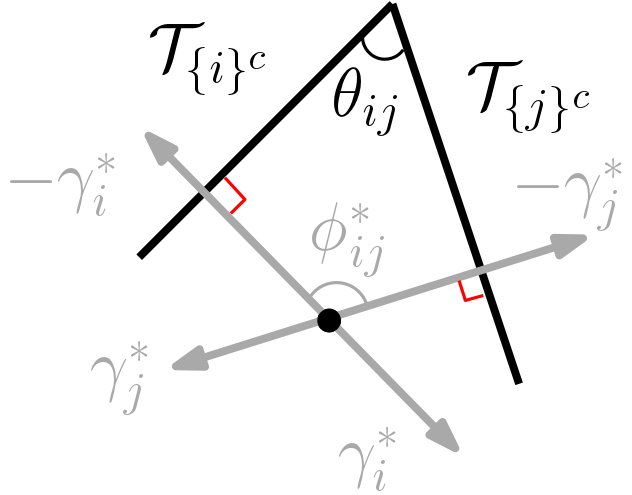
\includegraphics[scale=0.2]{angles}
	\caption{The angles in a simplex and its dual. The angle $\phi^\du_{ij}$ between $\bgamma^\du_i$ and $\bgamma^\du_i$ is the same as that between $-\bgamma_i^\du$ and $-\bgamma_j^\du$. From here  we  see that $\theta_{ij}+\phi^\du_{ij}=\pi$.}
\end{figure}
There are several angles worth discussing in a simplex. For a simplex $\ssplx$, let $\phi^\du_{ij}(\ssplx)$ be the angle between the outer normals to $\ssplx_\ic$ and $\ssplx_\jc$. As usual, the paranthetical $(\ssplx)$ will typically be dropped when the simplex is understood from context. Using the notion of the dual simplex introduced in the previous section, we can write 
 \begin{equation*}
\cos \phi^\du_{ij}(\ssplx) = \frac{\la \bgamma^\du_i,\bgamma^\du_j\ra }{\norm{\bgamma^\du_i}_2 \cdot \norm{\bgamma^\du_j}_2},
\end{equation*}
where $\{\bgamma^\du_i\}$ are the vertices of $\ssplx^\du$. The superscript represents  the fact that the angle is between the  vertices of the dual simplex. 
Now, define $\theta_{ij}(\ssplx)$ to be the angle between $\ssplx_\ic$ and $\ssplx_\jc$. Appealing to elementary geometry, we see that the angles $\phi^\du_{ij}$ and $\theta_{ij}$ are \emph{supplementary}, i.e., their sum is $\pi$. Hence, 
\begin{equation}
\label{eq:cos_theta_ij}
\cos \theta_{ij}(\ssplx) = - \frac{\la \bgamma^\du_i,\bgamma^\du_j\ra }{\norm{\bgamma^\du_i}_2 \cdot \norm{\bgamma^\du_j}_2},
\end{equation}
where we've used that $\cos(\phi^\du_{ij}) = \cos(\pi - \theta_{ij}) = -\cos(\theta_{ij})$. This allows us to define the notion of  hyperacuteness in simplices as follows. 

\begin{definition}
	\label{def:hyperacute}
	We call the simplex $\ssplx\subset \R^{n-1}$ \emph{hyperacute} if $\theta_{ij}(\ssplx)\leq \pi/2$ for all $i,j\in[n]$. If $\ssplx$ is not hyperacute, it is called \emph{obtuse}. 
\end{definition}


